Artificial intelligence has become the buzz word of modern computing. While the inner workings of most machine learning techniques are overlooked by many disciplines, the end results speak for themselves. Machine learning techniques allow for adaptable models that can be applied to a variety of problems, like decision trees or support vector machines \citep{somvanshi2016review}. Traditional statistical methods require a thorough understanding of the mathematics behind the algorithm, which can lead to an increase in the time to obtain a result. Machine learning algorithms do not require this level of understanding, but the reduced level of understanding required comes at the cost of interpretability. Parameters within models like Least Squares Regression can be interpreted directly, allowing for researchers to obtain a better understanding of what the model achieves. 

Deep learning is a term used to describe the use of neural networks to extract high-level features from data, and will be the focus of this paper (see Table \ref{tab:Definitions} for explanations of common terminology in this literature). These particular models involve an input layer, a hidden state comprised of 1 or more layers, and an output layer. A visualization of a neural network is shown in Figure \ref{fig:NueralNetwork}.

\begin{table}[hbt!]
\centering
\begin{tabular}{|p{0.35\linewidth} | p{0.55\linewidth}|}
    \hline
    Term & Definition \\
    \hline
    Deep Learning & The use of neural networks to extract high-level features from data.\\
    \hline
    Neural Network & A network of input nodes, a hidden layer(s), and an output node (Figure \ref{fig:NueralNetwork}).\\
    \hline
    Hidden Layer & A layer of nodes with activation functions used to extract features from the input layer. \\
    \hline
    Activation Functions & Functions that map the input to a specific range of values (i.e. between 0 and 1) (Figure \ref{fig:Activations}).\\
    \hline
    Backpropogation & Application of the chain rule used to approximate the gradient of error across parameter values. \\
    \hline 
    Exploding/Vanishing Gradient & A common issue in deep learning where the error gradient is difficult or impossible to approximate. \\
    \hline
    Recurrent Neural Network (RNN) & A sequence of Neural Networks that use sequential data as inputs (Figure \ref{fig:RNN}).\\
    \hline
    Long Short-Term Memory (LSTM) Network & A combination of cell states and memory cells set up similar to RNNs that minimize the issues with gradient descent (Figure \ref{fig:LSTM}). \\
    \hline
    Loss Function & A function that represents the error in a model (Mean Squared Error, Mean Absolute Error, etc.). These can differ based on the type of problem (quantitative or classification-based).\\
    \hline
    Batch & Number of inputs to be used for a single point prediction. \\
    \hline
    Hyperparameter & A parameter that is able to be tuned within a layer of a model. \\
    \hline
    Learning Rate & How quickly a model will adjust parameters when approximating optimal values. \\
    \hline
    Training/Testing Data & Partitions of the data used to train the model or assess performance, respectively. \\
    \hline
    
    \hline
\end{tabular}
\caption{Definitions of terms used throughout this paper.}
\label{tab:Definitions}
\end{table}

\begin{figure}[ht]
    \centering
    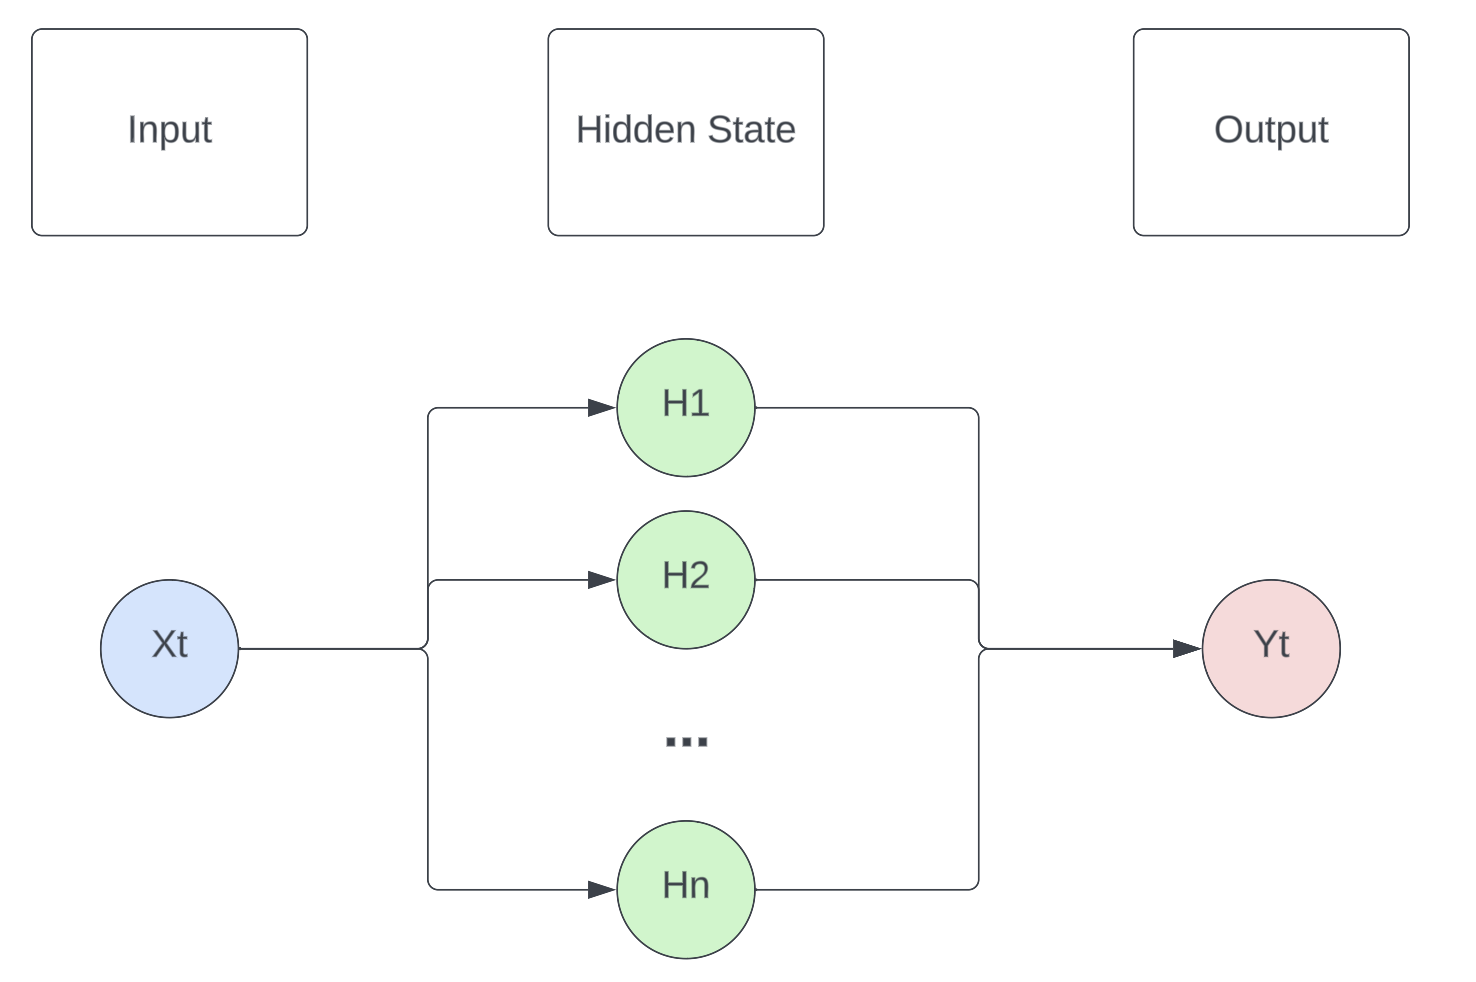
\includegraphics[width=0.8\linewidth]{"Figures/Traditional_NN.png"}
    \caption{A flowchart depicting a single-layer Neural Network. The input layer (blue) contains a single node, indicating a single value would be taken as an input. The hidden state (green) contains a single layer of \textit{n} nodes. The output layer (red) contains a single node, indicating a single value would be received as an output. Graphic made with LucidChart.}
    \label{fig:NueralNetwork}
\end{figure}

The nodes within a neural network, specifically within the hidden layer, take an input value from the input layer and apply an activation function, which are used to convert a given input to a value within a given range based on the activation function. A visualization is shown for the Linear, Rectified Linear Unit (ReLU), Sigmoid, and Hyperbolic Tangent (Tanh) activation functions in Figure \ref{fig:Activations}. This process is important as it allows for the outputs of each node to be normalized which can help with the training process for the weights and biases in the network. For example, if inputs were recorded as meters, a 1,000 meter input would have a larger impact on the output than if the units were recorded as kilometers.

\begin{figure}[ht]
    \centering
    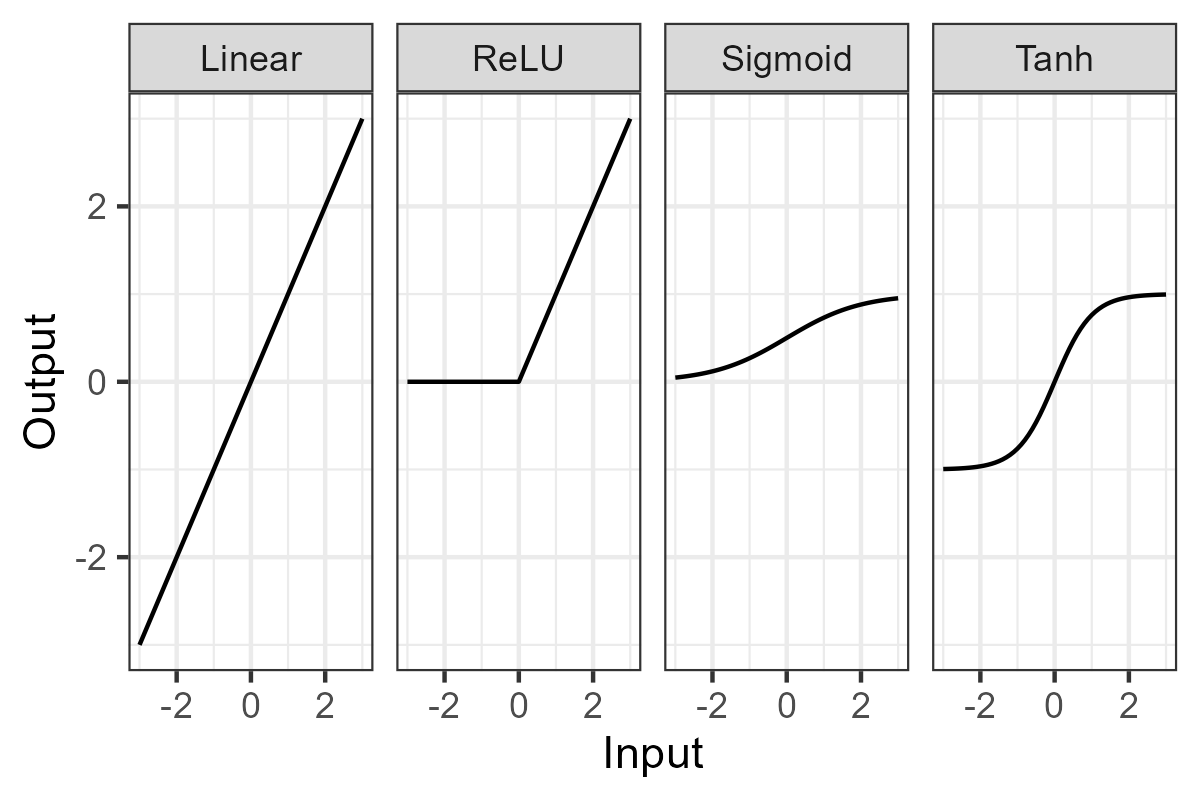
\includegraphics[width=0.8\linewidth]{"Figures/Activations.png"}
    \caption{A comparison of common activation functions. Note how the range of the inputs compares to the range of the outputs for different activations.}
    \label{fig:Activations}
\end{figure}

In addition to activation functions, each connection between nodes has a weight and bias. For example, the connection between $H_1$ and $X_t$ in Figure \ref{fig:NueralNetwork} would take the form:
\begin{equation*}
    H_1 = \sigma[w_1*X_t + b_1]
\end{equation*}
where $\sigma$ indicates the activation function being applied, $w_1$ indicates the weight, and $b_1$ indicates the bias. The weights and biases in a network are what get tuned in the training process.

Training of neural networks occurs through the process of backpropogation, which is an application of the chain rule in calculus to determine how the output changes based on the change of a single parameter, or trainable value (weights and biases) \citep{rojas1996backpropagation}. In practice, this means that the change in the prediction can be written as a function of the change in each parameter. The prediction of $y$ is compared to the observed value of $y$ in order to approximate a gradient, where each dimension represents a parameter. Then, gradient descent is used to find a minimum error, or loss, in the predictions.